\section{Aumentando Árboles Binarios}

Hasta ahora, el único uso que le podemos dar al Treap es como Conjunto / Diccionario. 
Esto no es útil para competencias, porque existen en las bibliotecas estándar implementaciones de estos tipos de datos. 
Por ejemplo, en C++ se puede usar \texttt{std::set} o \texttt{std::map}, respectivamente.

La idea va a ser \textit{aumentar} el árbol, almacenando información adicional en los nodos, para poder hacer operaciones más interesantes. 

\subsection[Árbol de Estadísticos de Orden (Order Statistics Tree)]{Árbol de Estadísticos de Orden \newline (Order Statistics Tree)}
\label{sec:order-statistics-tree}

Un Árbol de Estadísticos de Orden es un ABB, que además soporta las siguientes operaciones:

\begin{enumerate}
    \item Select(\(k\)), que retorna el \(k\)-ésimo elemento más chico.
    \item Rank(\(x\)), que devuelve la cantidad de elementos menores o iguales a \(x\).
\end{enumerate}

A la respuesta de Select(\(k\)) también se la llama \(k\)-ésimo estadístico de orden. Además, si \(x\) está en el conjunto, Rank(\(x\)) nos dice que número de estadístico de orden es \(x\).

Ambas operaciones van a funcionar en \(\mathcal{O}(\lg n)\), pero vamos a tener que guardar un parámetro adicional: el \textit{tamaño} de un subárbol.

Para cada nodo \(x\), definimos su tamaño como:
\[
|x| = |x_L| + |x_R| + 1
\]
donde \(x_L\) y \(x_R\) son sus hijos izquierdo y derecho.
Además, si un nodo \(x\) es nulo, decimos que su tamaño es cero.

Este valor adicional se puede mantener calculándolo al momento de creación, y actualizando un nodo cada vez que cambia alguno de sus hijos.
Para esto, podemos cambiarlo en Split() y Merge() cuando estamos por devolver el nuevo árbol.

\begin{center}
\begin{tikzpicture}[
level 1/.style={sibling distance=2in},
level 2/.style={sibling distance=1in},
level 3/.style={sibling distance=0.5in},
every node/.style={
    circle split,
    draw
}
]

\node { 26 \nodepart{lower} 7 }
    child {
        node { 17 \nodepart{lower} 4 }
        child { node { 4 \nodepart{lower} 1 } }
        child {
            node { 21 \nodepart{lower} 2 }
            child { node { 19 \nodepart{lower} 1} }
            child [missing]
        }
    }
    child {
        node { 41 \nodepart{lower} 2 }
        child { node { 30 \nodepart{lower} 1 } }
        child [missing]
    }
;
\end{tikzpicture}
\captionof{figure}{Clave y tamaño en un Order Statistics Tree}
\end{center}

\subsubsection{Select()}

Vamos a recorrer el árbol desde la raíz, comparando los tamaños con el \(k\) buscado.
Si el hijo izquierdo tiene exactamente \(k - 1\) nodos, entonces la respuesta es la raíz. Si tiene más de \(k - 1\), está en el hijo izquierdo, así que llamamos recursivamente. Finalmente, si tiene menos de \(k - 1\) nodos, la respuesta debe estar en el subárbol derecho, y llamamos a Select(\(k - |x_L| - 1\)) sobre el subárbol derecho.

\vbox{
\begin{minted}{c++}
int select(Treap root, int k) {
  if (size(root->left) == k - 1) return root->value;
  if (size(root->left) > k - 1) {
    return select(root->left, k);
  } else {
    k -= size(root->left) + 1;
    return select(root->right, k);
  }
}
\end{minted}
}

\subsubsection{Rank()}

Para implementar Rank(), partimos el Treap con respecto a \(x\), usando Split(). La respuesta es el tamaño de \(T_\leq\), lo único es que hay que recordar llamar a Merge() antes de retornar.

\subsection{SPOJ - Ghost Town}

\problema{
\textbf{Ghost Town:}

Queremos un multiconjunto que soporte:

\begin{enumerate}
\item Count(\(x\)): retorna cantidad de valores \(\leq x\)
\item Select(\(k\)): retorna el \(k\)-ésimo valor más chico
\item Insert(\(x\) + Count(\(x\)))
\end{enumerate}

En todos los casos, los elementos se cuentan con repeticiones.
Por ejemplo, Select(\(\{1, 1, 2\}, 2\)) = 1.

\url{https://www.spoj.com/problems/COUNT1IT/}
}

Notar que, si en lugar de un multiconjunto pidiera un conjunto, sería simplemente implementar un Order Statistics Tree.
Aunque es tentador que nuestra implementación permita nodos con valores repetidos, esto nos da de peor caso \(h = \mathcal{O}(n)\), insertando siempre el mismo elemento\footnote{Esto es similar a ciertas implementaciones de Quicksort, que resultan \(\mathcal{O}(n^2)\) si todos los elementos son iguales.}.

En su lugar vamos a guardar en cada nodo la cantidad de veces que aparece su valor en el multiconjunto, y lo notamos \(x_f\). Es suficiente cambiar nuestra definición de tamaño a

\[|x| = |x_L| + |x_R| + |x_f|\]

así como modificar ligeramente la implementación de Select(), y sumarle uno a \(x_f\) al insertar un valor repetido.

\subsection{SPOJ - Ada and Harvest}

\problema{
\textbf{Ada and Harvest:}

Tenemos una lista \(a_1, \dots, a_n\) de números, y queremos responder \(q\) consultas del tipo ``contar cuántos números en \(a_1, ..., a_{k - 1}\) iguales a \(x\), y luego reemplazar \(a_k\) por \(x\)''.

\url{https://www.spoj.com/problems/ADACROP/}
}

Vamos a tratar de adaptar el problema para poder usar un Order Statistics Tree.
Notar que dos números distintos en la lista ``no interactúan'' entre sí, porque al momento de responder para \(x\), 
sólo nos interesan las posiciones con valor igual a \(x\).

\begin{center}
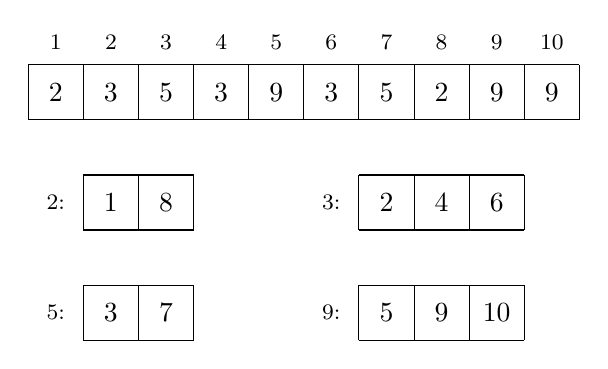
\begin{tikzpicture}[scale=0.7]
\draw (0,0) grid (10,1);

\node at (0.5,0.5) {$2$};
\node at (1.5,0.5) {$3$};
\node at (2.5,0.5) {$5$};
\node at (3.5,0.5) {$3$};
\node at (4.5,0.5) {$9$};
\node at (5.5,0.5) {$3$};
\node at (6.5,0.5) {$5$};
\node at (7.5,0.5) {$2$};
\node at (8.5,0.5) {$9$};
\node at (9.5,0.5) {$9$};

\footnotesize
\node at (0.5,1.4) {$1$};
\node at (1.5,1.4) {$2$};
\node at (2.5,1.4) {$3$};
\node at (3.5,1.4) {$4$};
\node at (4.5,1.4) {$5$};
\node at (5.5,1.4) {$6$};
\node at (6.5,1.4) {$7$};
\node at (7.5,1.4) {$8$};
\node at (8.5,1.4) {$9$};
\node at (9.5,1.4) {$10$};

\normalsize
\draw (1,-1) grid (3, -2);
\node at (1.5, -1.5) {$1$};
\node at (2.5, -1.5) {$8$};

\footnotesize
\node at (0.5, -1.5) {$2$:};

\normalsize
\draw (6,-1) grid (9, -2);
\node at (6.5, -1.5) {$2$};
\node at (7.5, -1.5) {$4$};
\node at (8.5, -1.5) {$6$};

\footnotesize
\node at (5.5, -1.5) {$3$:};

\normalsize
\draw (1,-3) grid (3, -4);
\node at (1.5, -3.5) {$3$};
\node at (2.5, -3.5) {$7$};

\footnotesize
\node at (0.5, -3.5) {$5$:};

\normalsize
\draw (6,-3) grid (9, -4);
\node at (6.5, -3.5) {$5$};
\node at (7.5, -3.5) {$9$};
\node at (8.5, -3.5) {$10$};

\footnotesize
\node at (5.5, -3.5) {$9$:};

\end{tikzpicture}
\captionof{figure}{Descomposición en índices del ejemplo}
\end{center}

Por esta razón, vamos a armar un árbol por cada valor, y guardamos los índices 
en los que aparece este valor en la lista actual. 
Aunque esto parezca costoso, vamos a ver a lo sumo \(n + q\) valores distintos, y podemos guardar los árboles en un diccionario.

Ahora, responder una consulta es buscar el árbol apropiado y llamar a Rank(\(k\)), y después sacar \(k\) del árbol viejo, y añadirlo al nuevo. Por lo tanto, la complejidad es \(\mathcal{O}((n + q) \lg (n + q))\).